\documentclass[11pt,a4paper]{article}

\usepackage[utf8]{inputenc}
\usepackage[T1]{fontenc}
\usepackage{lmodern}
\usepackage[french]{babel}
\usepackage[margin=2.1cm]{geometry}
\usepackage{amsmath,amssymb}
\usepackage{booktabs,tabularx,array,multirow}
\usepackage{graphicx}
\usepackage[table]{xcolor}
\usepackage{tikz}
\usetikzlibrary{arrows.meta,positioning}
\usepackage{tcolorbox}
\tcbuselibrary{skins,breakable}
\usepackage{enumitem}
\usepackage{caption}
\usepackage{float}
\usepackage{fancyhdr}
\usepackage[hidelinks]{hyperref}

\graphicspath{{../reports/figures/}}

\definecolor{bleu}{HTML}{1F4E79}
\definecolor{bleuclair}{HTML}{E8F0F8}
\definecolor{vert}{HTML}{2E7D32}
\definecolor{vertclair}{HTML}{E8F5E9}
\definecolor{orange}{HTML}{E65100}
\definecolor{orangeclair}{HTML}{FFF3E0}

\newtcolorbox{constat}[1][]{colback=vertclair,colframe=vert,fonttitle=\bfseries,title={#1},breakable}
\newtcolorbox{limite}[1][]{colback=orangeclair,colframe=orange,fonttitle=\bfseries,title={#1},breakable}
\newcommand{\best}[1]{\textbf{#1}}
\setlist{itemsep=1pt,topsep=3pt}
\renewcommand{\arraystretch}{1.12}
\captionsetup{font=small}

\pagestyle{fancy}
\fancyhf{}
\lhead{\small CAMELYON17 — détection de métastases et stade pN}
\rhead{\small \thepage}
\setlength{\headheight}{14pt}

\title{\vspace{-1.4cm}\textbf{\color{bleu}Détection de métastases ganglionnaires\\et stade pN du cancer du sein (CAMELYON17)}\\[4pt]
\large Robustesse au changement d'hôpital : des CNN aux modèles de fondation}
\author{Ali Houaoui \;—\; \emph{[noms des autres membres de l'équipe]}}
\date{Rapport de projet — 26 novembre 2026\\
\small Code : dépôt GitHub \texttt{alihouaoui/Projet\_Camelyon17} (journal de bord : \texttt{JOURNAL.md})}

\begin{document}
\maketitle
\thispagestyle{fancy}

\begin{abstract}
\noindent Nous cherchons à détecter les métastases du cancer du sein sur des lames de ganglions lymphatiques, puis à en déduire le
\emph{stade pN} de chaque patiente, avec une contrainte centrale : le modèle doit rester fiable dans un \textbf{hôpital qu'il n'a
jamais vu}. Sur les 455\,954 patchs de Camelyon17-WILDS (5 hôpitaux), découpés par patiente, nous comparons \textbf{huit
classifieurs} : deux références « couleur + texture », un petit CNN, un ResNet18 pré-entraîné, et quatre modèles de fondation
figés suivis d'une régression logistique. Le seuil de décision est fixé sur les hôpitaux d'entraînement (sensibilité 95\,\%)
puis appliqué tel quel. Le ResNet18 classe bien les patchs de l'hôpital de test (AUC 0,958) mais n'y détecte que \textbf{69\,\%} des
tumeurs ; un modèle de fondation de pathologie (Phikon) atteint une AUC de 0,990 et une sensibilité de \textbf{98\,\%}.
L'exploration montre pourquoi : la couleur seule identifie l'hôpital dans 80\,\% des cas. Une augmentation de couleur
(HED) fait passer le petit CNN de 82 à 95\,\% de sensibilité sur l'hôpital de test, mais aide peu le ResNet18. Pour le stade pN de 57 patientes
jamais vues (285 lames entières lues à distance), nous comparons une règle de taille, une forêt aléatoire et un modèle
multi-instances à attention (ABMIL) : l'ABMIL hybride atteint un kappa quadratique de \textbf{0,89} contre 0,80 (écart
+0,08, IC 95\,\% [0,01 ; 0,18]). Les micro-métastases restent le point faible. Nous discutons l'interprétabilité (Grad-CAM,
cartes de chaleur), le changement de domaine et les enjeux éthiques d'un tel outil.
\end{abstract}

\tableofcontents

%=====================================================================
\section{Contexte et objectifs}
%=====================================================================

\paragraph{Le problème médical.}
Dans le cancer du sein, l'atteinte des ganglions lymphatiques de l'aisselle est l'un des principaux facteurs pronostiques.
Chaque ganglion retiré est coupé, coloré à l'hématoxyline-éosine (H\&E : noyaux violets, cytoplasme rose) et numérisé en une
\emph{lame entière} (WSI) d'environ $100\,000\times200\,000$ pixels. Le pathologiste y cherche des cellules tumorales et mesure
la plus grande lésion : \emph{ITC} ($<0{,}2$\,mm), \emph{micro-métastase} (0,2–2\,mm) ou \emph{macro-métastase} ($>2$\,mm).
Les 5 ganglions d'une patiente donnent son \textbf{stade pN} (pN0, pN0(i+), pN1mi, pN1, pN2), qui oriente le traitement.
L'examen est long et les petites lésions sont facilement manquées : c'est un cas d'usage classique de l'aide au diagnostic.

\paragraph{Coût asymétrique des erreurs.} Une métastase ratée (faux négatif) peut priver une patiente d'un traitement ; une fausse
alerte coûte une relecture. Toutes nos métriques et nos choix de seuil découlent de cette asymétrie.

\paragraph{Objectifs.}
\begin{enumerate}
  \item \textbf{Étape 1 — détection} : classer chaque patch ($96\times96$ pixels) en tumoral / non tumoral, et \textbf{comparer
        plusieurs familles de modèles}, en mesurant surtout leur comportement sur des \textbf{hôpitaux jamais vus}.
  \item \textbf{Étape 2 — stade} : appliquer le meilleur détecteur aux lames entières, en déduire la classe de chaque ganglion
        puis le stade pN, et comparer trois méthodes d'agrégation.
  \item \textbf{Étape 3 — recul critique} : changement de domaine, interprétabilité, éthique.
\end{enumerate}

\paragraph{Pourquoi CAMELYON17 ?} (i) Tâche clinique réelle avec des règles officielles (on peut construire le stade comme le
pathologiste) ; (ii) \textbf{5 hôpitaux néerlandais} aux scanners et colorations différents : cas d'école du changement de
domaine ; (iii) deux niveaux de données (patchs prêts à l'emploi et lames entières avec stades) ; (iv) références publiées
(challenge : Bándi et al., 2019 ; benchmark WILDS : Koh et al., 2021).

%=====================================================================
\section{Données}
%=====================================================================

\subsection{Patchs Camelyon17-WILDS (étape 1)}
\textbf{455\,954 patchs} RGB de $96\times96$ pixels (niveau 2 de la pyramide, $\approx$\,0,97\,µm/pixel, soit $\approx$\,93\,µm de tissu),
issus de \textbf{50 lames, 43 patientes, 5 hôpitaux} (10 lames annotées par hôpital). Étiquette : 1 si le centre du patch tombe dans
un contour tumoral tracé par un pathologiste. Le serveur officiel ayant un certificat HTTPS expiré, nous avons utilisé le miroir
Hugging Face \texttt{wltjr1007/Camelyon17-WILDS} (21 fichiers Parquet, 10,7\,Go), dont nous avons vérifié les effectifs.

\subsection{Exploration}
\begin{itemize}
  \item \textbf{Qualité} : format homogène ($96\times96\times3$, entiers 0–255), aucune valeur manquante.
  \item \textbf{Classes} : équilibrées ($\approx$\,50/50) \emph{par construction de WILDS}. Sur une vraie lame, le tissu tumoral
        représente souvent moins de 1\,\% : l'exactitude serait alors trompeuse, d'où le choix de la sensibilité.
  \item \textbf{Couleur et hôpital} : six statistiques de couleur (moyennes RVB, saturation, hématoxyline, éosine) suffisent à une
        régression logistique pour \textbf{reconnaître l'hôpital dans 80\,\% des cas} (hasard : 20\,\%). L'hôpital 2 est nettement plus
        violet et saturé (figure~\ref{fig:eda}). Un modèle risque donc d'apprendre la « signature » de couleur de ses hôpitaux
        plutôt que la morphologie des cellules.
  \item \textbf{Dépendance spatiale} : les patchs tumoraux d'une lame sont regroupés ; deux patchs voisins sont presque identiques
        (figure~\ref{fig:pos}).
\end{itemize}

\begin{figure}[H]
\centering
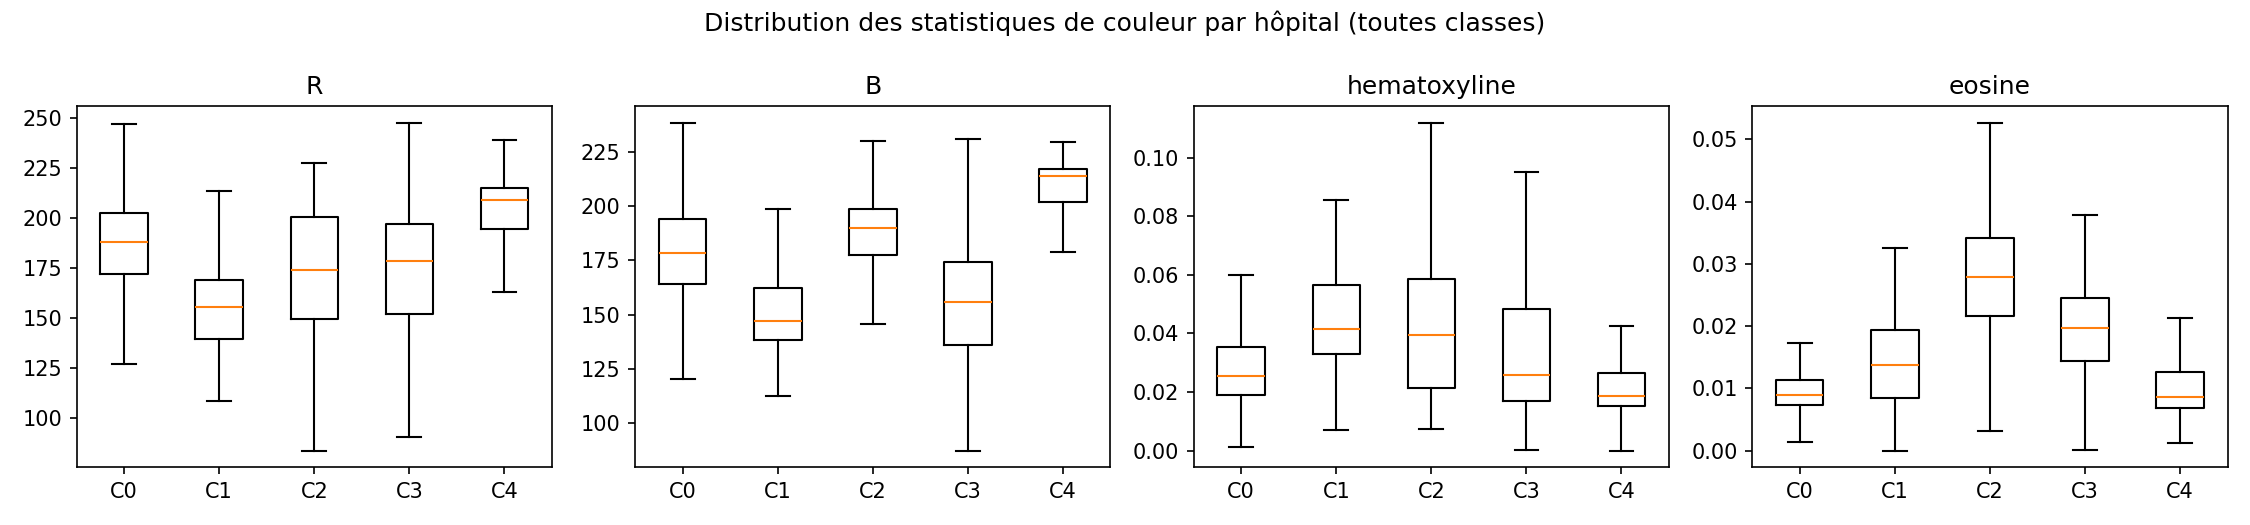
\includegraphics[width=0.49\textwidth]{couleur_par_centre.png}\hfill
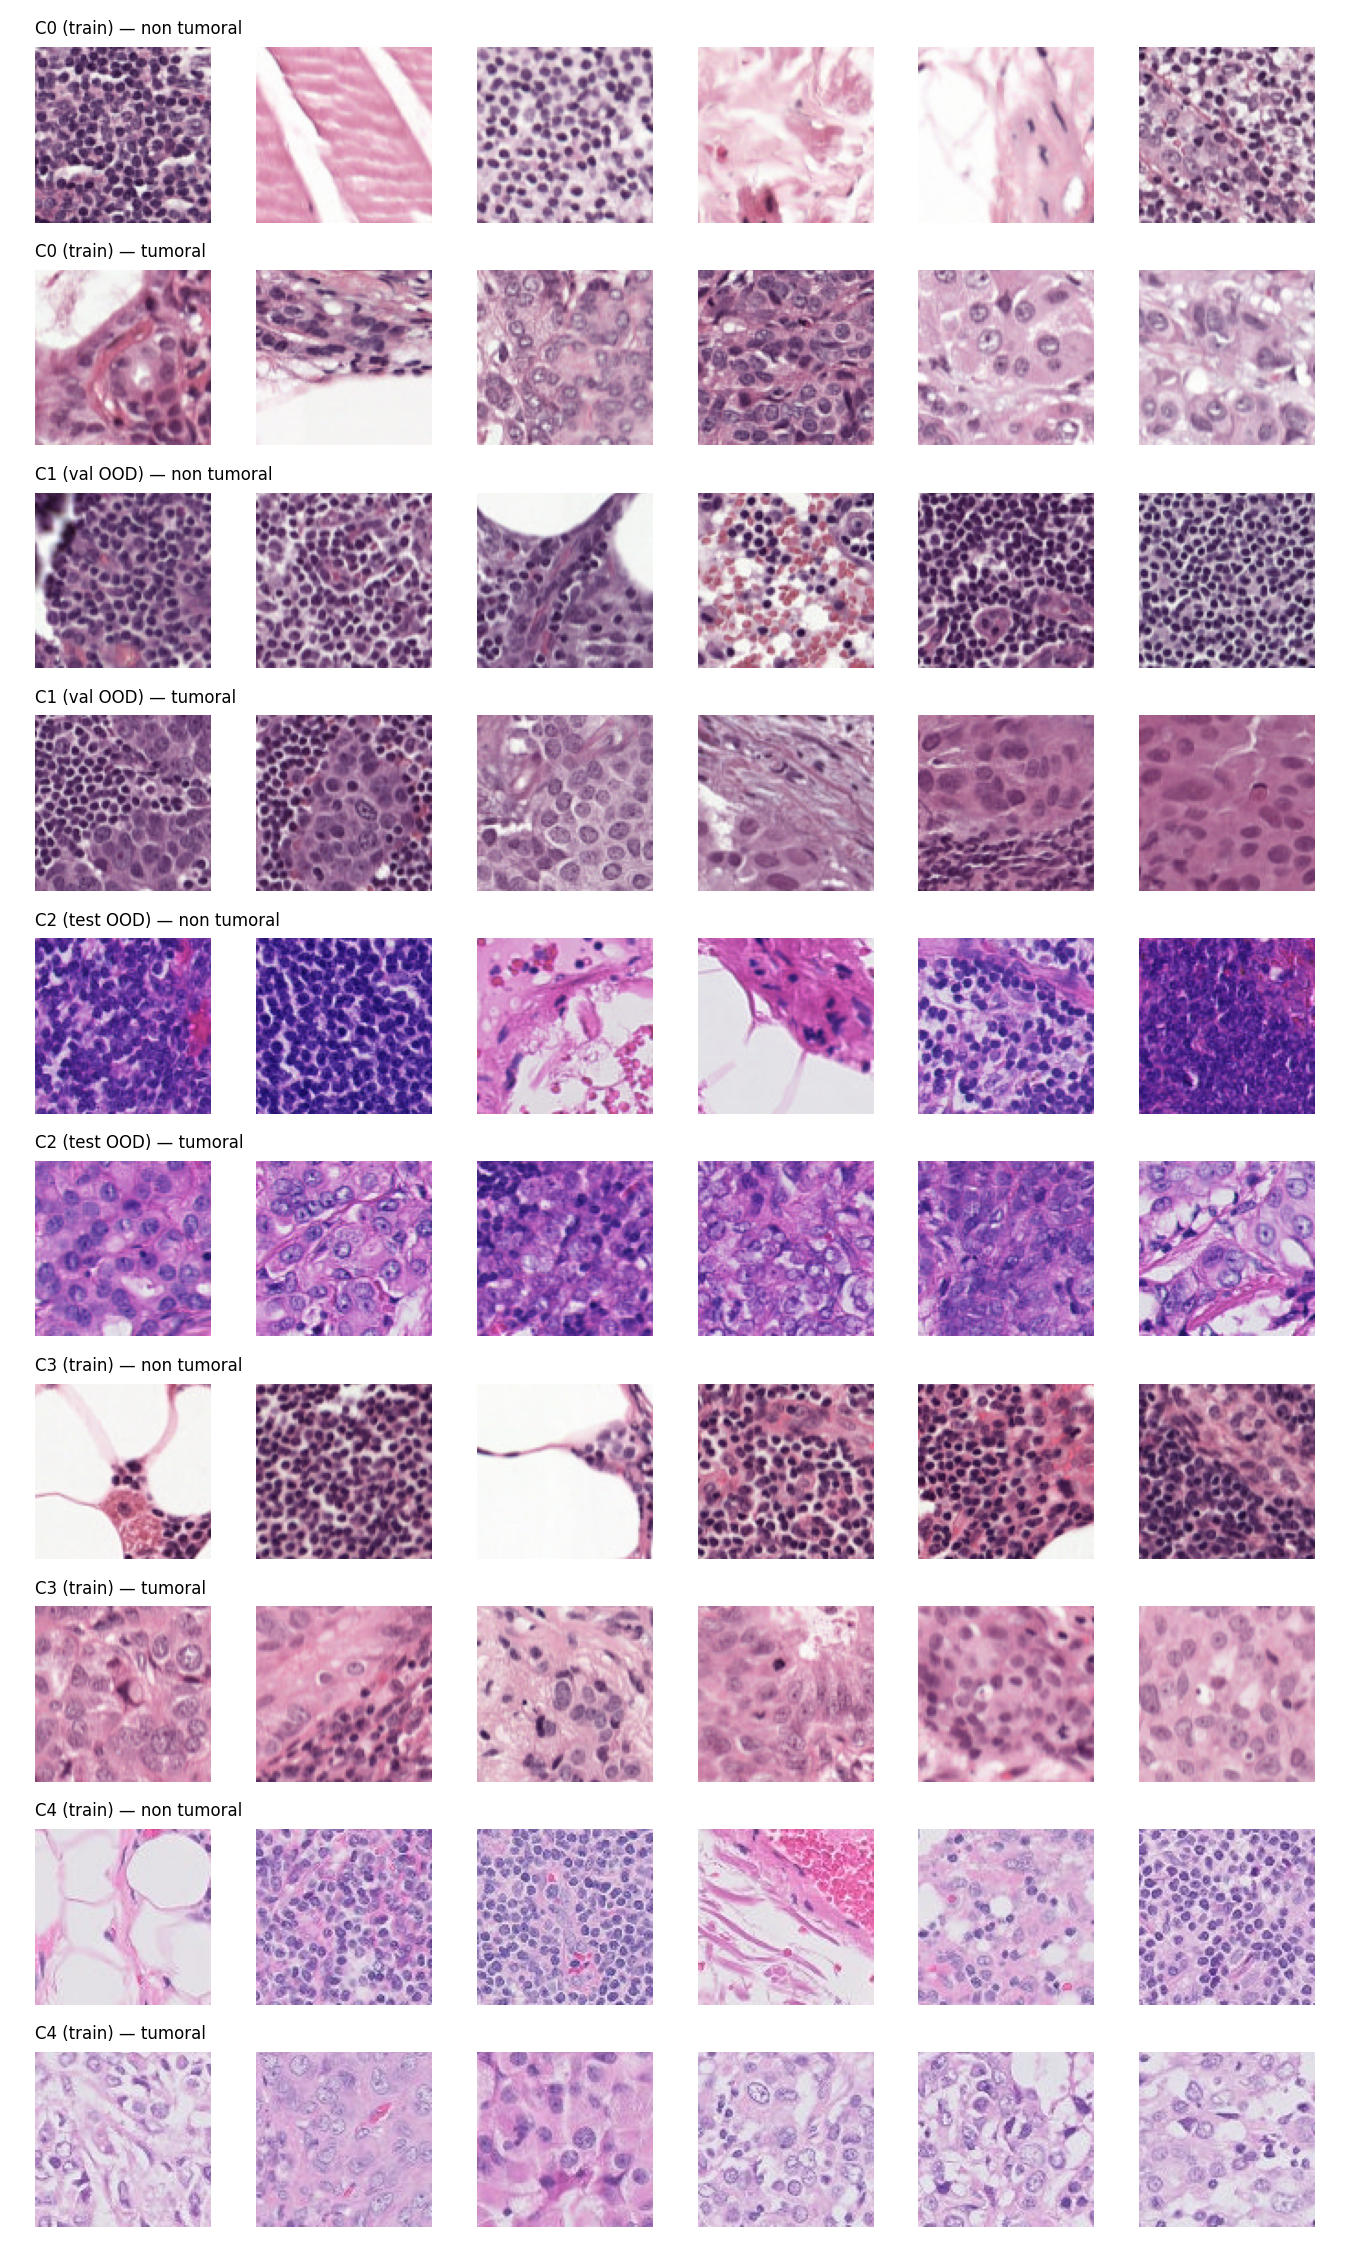
\includegraphics[width=0.49\textwidth]{galerie.png}
\caption{À gauche : distribution de la couleur par hôpital. À droite : patchs non tumoraux et tumoraux par hôpital.}
\label{fig:eda}
\end{figure}

\begin{figure}[H]
\centering
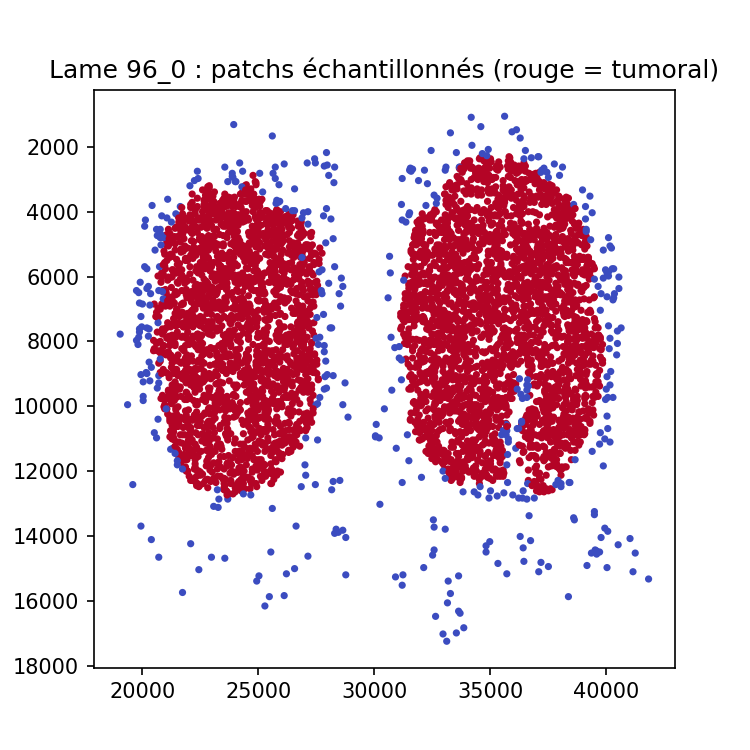
\includegraphics[width=0.40\textwidth]{positions_lame.png}\hfill
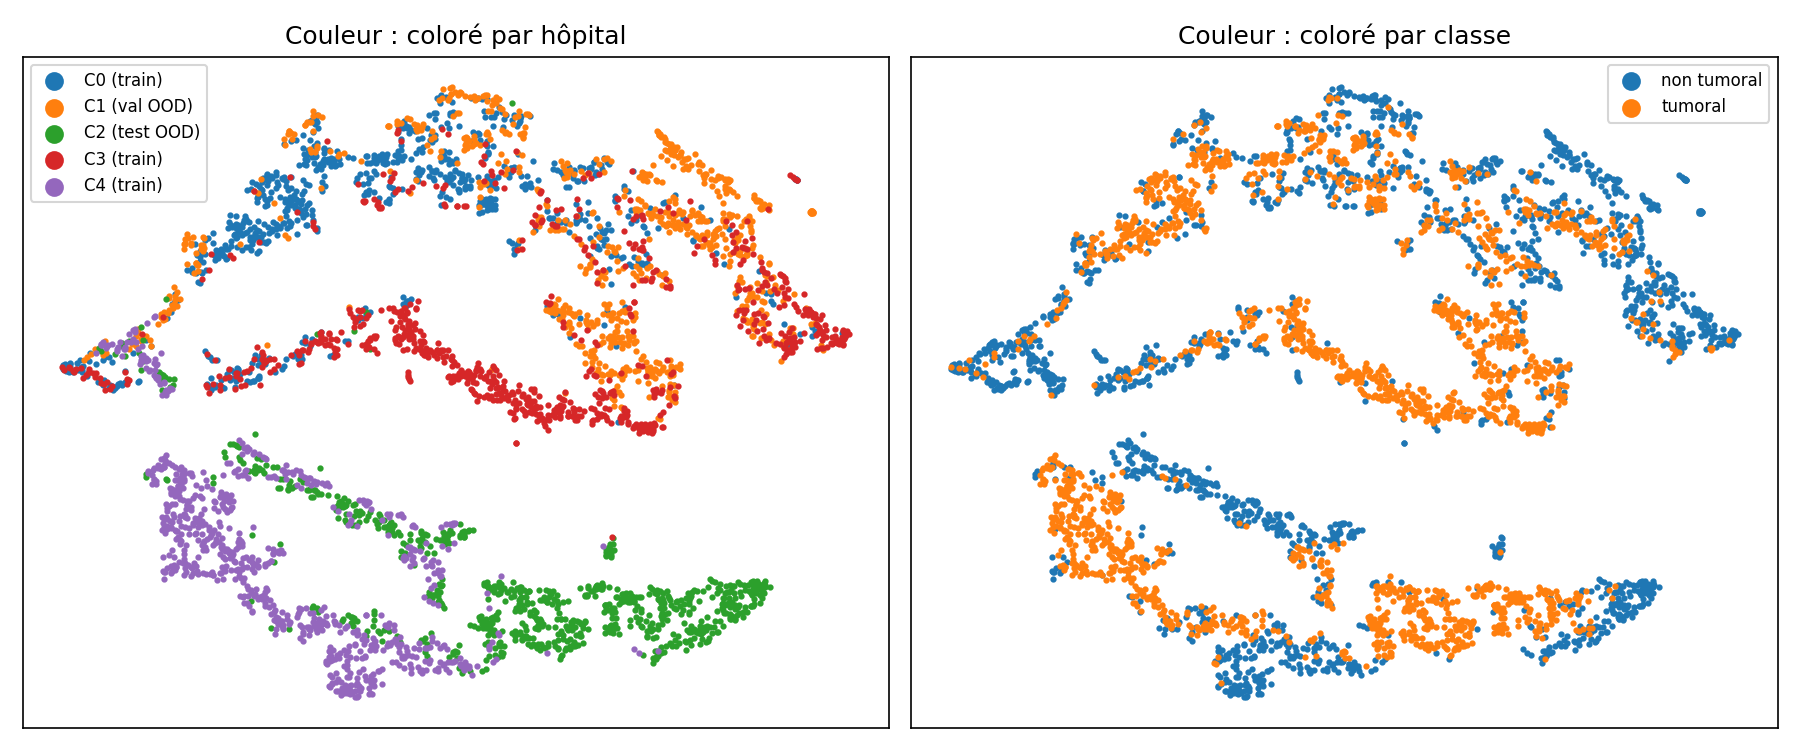
\includegraphics[width=0.53\textwidth]{tsne_couleur.png}
\caption{À gauche : position des patchs dans une lame (rouge : tumoral) ; les tumeurs forment des zones continues. À droite :
projection t-SNE des statistiques de couleur, colorée par hôpital ; les hôpitaux forment des groupes distincts.}
\label{fig:pos}
\end{figure}

\subsection{Découpage sans fuite}
Les deux constats précédents imposent le découpage : \textbf{par patiente} (pour éviter des quasi-copies entre entraînement et test)
et \textbf{par hôpital} (pour mesurer la généralisation à un hôpital inconnu).

\begin{table}[H]
\centering\small
\begin{tabularx}{\textwidth}{lllX}
\toprule
\textbf{Ensemble} & \textbf{Contenu} & \textbf{Patchs} & \textbf{Usage} \\
\midrule
\texttt{train} & hôpitaux 0, 3, 4 — 80\,\% des patientes & 283\,794 & apprentissage des poids \\
\texttt{val\_id} & hôpitaux 0, 3, 4 — 20\,\% des patientes & 52\,202 & choix de l'époque et du seuil \\
\texttt{val\_ood} (C1) & hôpital 1, jamais vu & 34\,904 & généralisation, critère principal \\
\texttt{test\_ood} (C2) & hôpital 2, jamais vu & 85\,054 & test final \\
\bottomrule
\end{tabularx}
\caption{Découpage (choix des hôpitaux identique au benchmark WILDS). Le split \texttt{id\_val} officiel de WILDS reprend des
patchs des mêmes lames que l'entraînement : il est écarté. Une fonction refuse tout découpage où une patiente apparaît deux fois.}
\end{table}

\noindent\textbf{Faiblesse identifiée en cours de projet} : \texttt{val\_id} ne compte que 5 patientes et 99\,\% de ses patchs
tumoraux viennent de 2 patientes de l'hôpital 3. Pour les modèles de fondation, le seuil a donc été choisi par validation croisée
groupée par patiente (5 plis) sur les hôpitaux 0, 3 et 4 (section~\ref{sec:fm}).

\subsection{Lames entières (étape 2)}
Lames CAMELYON17 du bucket public AWS et fichier officiel \texttt{stages.csv}. Cohorte : les \textbf{57 patientes dont le détecteur
n'a vu aucune image} (les 43 patientes WILDS sont exclues), soit \textbf{285 lames} et $\approx$\,3 millions de tuiles :
24 pN0, 3 pN0(i+), 9 pN1mi, 14 pN1, 7 pN2 ; 205 ganglions négatifs, 10 ITC, 27 micro, 43 macro. Les lames (1–3\,Go) ne sont pas
téléchargées : seules les tuiles recouvrant du tissu sont lues par requêtes HTTP « Range ».

%=====================================================================
\section{Méthodes}
%=====================================================================

\subsection{Étape 1 : huit classifieurs de patchs}
\begin{description}[style=nextline,leftmargin=0.4cm]
  \item[Références classiques (2 modèles)] statistiques de couleur et de texture (histogrammes, LBP, co-occurrence) puis
        \textbf{régression logistique} ou \textbf{forêt aléatoire}. Point de comparaison sans apprentissage profond.
  \item[Petit CNN (appris de zéro)] 4 blocs \{convolution $3\times3$, normalisation de lot, ReLU, max-pooling $2\times2$\} de largeurs
        32, 64, 128, 256, puis pooling global, dropout 0,3 et couche linéaire (389\,410 paramètres).
  \item[ResNet18 pré-entraîné] réseau résiduel de 18 couches (11\,M paramètres) pré-entraîné sur ImageNet ; dernière couche remplacée
        (2 sorties) et réseau entièrement ré-entraîné (\emph{fine-tuning}).
  \item[Modèles de fondation figés + sonde linéaire (4 modèles)] un Vision Transformer pré-entraîné par auto-supervision transforme
        chaque patch (agrandi à $224\times224$) en un vecteur ; une régression logistique décide. \textbf{Phikon} (ViT-B, 86\,M, TCGA),
        \textbf{Phikon-v2} (ViT-L, TCGA + CPTAC + GTEx), \textbf{Midnight-12k} (ViT-g, TCGA ; 100\,000 patchs par manque de temps de calcul)
        et, en contrôle, \textbf{DINOv2-base} (photos ordinaires). Aucun n'a vu CAMELYON lors de son pré-entraînement (fiches des modèles).
\end{description}

\paragraph{Entraînement des CNN.} Entropie croisée (non pondérée : classes équilibrées), AdamW (\emph{weight decay} $10^{-4}$),
calendrier OneCycle, lots de 256 patchs, augmentation par symétries et rotations de 90° (le tissu n'a pas d'orientation),
normalisation des entrées. Petit CNN : $\mathrm{lr}=10^{-3}$, 5 époques ; ResNet18 : $\mathrm{lr}=3\cdot10^{-4}$, 3 époques.
L'époque retenue est celle de meilleure AUC sur \texttt{val\_id} ; l'hôpital 2 n'est jamais évalué pendant l'entraînement.
\textbf{Expérience complémentaire} (section~\ref{sec:hed}) : mêmes réglages avec une augmentation de couleur \emph{HED-light}
(Tellez et al., 2019).

\subsection{Étape 2 : du patch au stade pN}
\begin{figure}[H]
\centering
\begin{tikzpicture}[node distance=0.45cm and 0.42cm, every node/.style={font=\small},
  box/.style={draw=bleu, fill=bleuclair, rounded corners, align=center, minimum height=1cm, text width=2.35cm},
  arr/.style={-{Stealth[length=2.3mm]}, thick, bleu}]
\node[box] (wsi) {Lame entière\\(1 ganglion)};
\node[box, right=of wsi] (tiles) {Tuiles $96{\times}96$\\sur le tissu};
\node[box, right=of tiles] (phikon) {Phikon figé\\+ sonde};
\node[box, right=of phikon] (map) {Carte de chaleur\\$p(\text{tumeur})$};
\node[box, below=0.9cm of map, fill=vertclair, draw=vert] (cls) {Classe du\\ganglion};
\node[box, left=of cls, fill=vertclair, draw=vert] (pn) {Règles pN\\(5 ganglions)};
\node[box, left=of pn, fill=orangeclair, draw=orange] (stage) {Stade pN\\de la patiente};
\draw[arr] (wsi) -- (tiles); \draw[arr] (tiles) -- (phikon); \draw[arr] (phikon) -- (map);
\draw[arr] (map) -- node[right, align=left, font=\scriptsize]{règle, forêt\\ou ABMIL} (cls);
\draw[arr] (cls) -- (pn); \draw[arr] (pn) -- (stage);
\end{tikzpicture}
\caption{Le stade n'est pas « deviné » par un modèle : il est construit comme le fait le pathologiste.}
\end{figure}

\begin{description}[style=nextline,leftmargin=0.4cm]
  \item[Carte de chaleur] masque de tissu (Otsu sur la saturation), toutes les tuiles du niveau 2 contenant au moins 25\,\% de tissu,
        notées par Phikon + sonde de l'étape 1.
  \item[(a) Règle de taille] tuiles au-dessus d'un seuil $t$, taches d'au moins $m$ tuiles, plus grand diamètre (Feret) en mm, puis
        seuils TNM 0,2 et 2\,mm \emph{non réglés} ; seuls $t$ et $m$ sont appris. Entièrement explicable.
  \item[(b) Forêt aléatoire] 300 arbres sur des résumés de la carte (probabilité maximale, nombre de tuiles et diamètre à plusieurs
        seuils, quantité de tissu) : l'approche des gagnants du challenge.
  \item[(c) ABMIL] apprentissage multi-instances à attention à porte (Ilse et al., 2018) : une lame est un « sac » de vecteurs Phikon,
        $z=\sum_k a_k h_k$ avec des poids d'attention $a_k$ appris ($\approx$\,110\,k paramètres). L'attention fait une moyenne pondérée et
        ne mesure pas une taille : le \textbf{modèle principal, fixé avant les résultats, est un ABMIL hybride} qui décide seulement
        « ganglion atteint ou non », la taille venant de la règle (a). Variante secondaire : ABMIL à 3 classes.
\end{description}

\subsection{Métriques et protocole d'évaluation}
\begin{itemize}
  \item \textbf{Sensibilité} $\frac{VP}{VP+FN}$ (tumeurs détectées), \textbf{métrique prioritaire} ; \textbf{spécificité}
        $\frac{VN}{VN+FP}$ (fausses alertes évitées) ; \textbf{AUC ROC} : probabilité qu'un patch tumoral reçoive un score plus élevé
        qu'un patch sain — elle juge le \emph{rangement}, indépendamment du seuil.
  \item \textbf{Seuil transféré} : réglé sur les hôpitaux d'entraînement pour une sensibilité de 95\,\%, puis appliqué \emph{tel quel}
        aux hôpitaux 1 et 2, comme dans un vrai déploiement où l'on ne peut pas régler le seuil sur les patientes à diagnostiquer.
  \item \textbf{Incertitude} : intervalles de confiance à 95\,\% par \textbf{bootstrap des patientes} (1\,000 tirages ; les patchs
        d'une patiente sont trop corrélés pour être ré-échantillonnés individuellement).
  \item \textbf{Étape 2} : \textbf{kappa de Cohen pondéré quadratique}, la métrique officielle,
        \[ \kappa=1-\frac{\sum_{ij} w_{ij}O_{ij}}{\sum_{ij} w_{ij}E_{ij}}, \qquad w_{ij}=\frac{(i-j)^2}{16}, \]
        où $O$ est la matrice de confusion observée et $E$ celle attendue par hasard ; puis le stade exact, et trois métriques cliniques en nombre de
        patientes : métastatiques ratées, macro ratées (erreur la plus grave), sur-stadification. Validation croisée par patiente,
        stratifiée sur le stade, 3 plis $\times$ 10 répétitions, \textbf{mêmes plis pour toutes les méthodes} ; écarts appariés avec
        IC par bootstrap des patientes.
  \item \textbf{Hygiène statistique} : chaque plan d'expérience a été écrit et critiqué \emph{avant} lancement ; les analyses imaginées
        après coup sont signalées comme exploratoires.
\end{itemize}

\paragraph{Calcul.} Mise au point sur Mac (échantillon de 40\,254 patchs) ; jeu complet sur \textbf{Google Colab gratuit} (GPU T4,
12,7\,Go de RAM), piloté depuis le Mac. Solutions aux contraintes : images décodées une fois dans un fichier lu à la demande
(\emph{memmap}, 12,6\,Go), points de sauvegarde rapatriés toutes les 4 minutes contre les coupures de session, augmentations faites
par lot sur le GPU (395 $\to$ 250\,s par époque), lecture partielle des lames à distance.

%=====================================================================
\section{Résultats — étape 1 : détection sur patchs}
%=====================================================================

\subsection{Références, CNN et ResNet18}
\begin{table}[H]
\centering\footnotesize\setlength{\tabcolsep}{4pt}
\begin{tabular}{lcccccc}
\toprule
\textbf{Modèle} & \textbf{AUC val\_id} & \textbf{AUC C1} & \textbf{AUC C2} & \textbf{Sens. C2} & \textbf{Spéc. C2} & \textbf{Ratées C2} \\
\midrule
Couleur + texture, rég. log. & 0,973 & 0,838 & 0,660 & 0,63 & 0,62 & 37\,\% \\
Couleur + texture, forêt & 0,965 & 0,901 & 0,896 & \best{0,99} & 0,36 & 1\,\% \\
Petit CNN (5 époques) & 0,993 & 0,912 & 0,893 & 0,82 & 0,79 & 18\,\% \\
ResNet18 (3 époques) & \best{0,997} & \best{0,979} & \best{0,958} & 0,69 & \best{0,99} & 31\,\% \\
\bottomrule
\end{tabular}
\caption{Jeu complet. Seuil fixé sur \texttt{val\_id} (sensibilité 95\,\%) puis appliqué tel quel. Références classiques entraînées
sur 30\,000 patchs et évaluées sur 20\,000 patchs par ensemble.}
\label{tab:cnn}
\end{table}

\begin{constat}[Un bon AUC ne suffit pas]
Le ResNet18 range le mieux les patchs de l'hôpital 2 (AUC 0,958) mais, au seuil appris ailleurs, il \textbf{rate 31\,\% des tumeurs}
(13\,183 sur 42\,527). Pour retrouver 95\,\% de sensibilité sur cet hôpital, il faudrait un seuil de 0,023 au lieu de 0,843 : ses
probabilités sont décalées vers « non tumoral ». Les modèles « couleur » ne transfèrent pas (régression logistique : AUC 0,66) ;
la forêt garde la sensibilité au prix de 64\,\% de fausses alertes. Enfin, \textbf{entraîner plus longtemps spécialise} : l'AUC du
ResNet18 sur l'hôpital 1 passe de 0,983 (époque 1) à 0,958 (époque 3) pendant que \texttt{val\_id} reste à 0,996.
\end{constat}

\subsection{Modèles de fondation figés}\label{sec:fm}
\begin{table}[H]
\centering\footnotesize\setlength{\tabcolsep}{4pt}
\begin{tabular}{lcccr}
\toprule
\textbf{Modèle (hôpital 2, 9 patientes)} & \textbf{AUC [IC 95\,\%]} & \textbf{Sensibilité [IC 95\,\%]} & \textbf{Spécificité} & \textbf{Tumeurs ratées} \\
\midrule
Petit CNN & 0,893 [0,74–0,94] & 0,82 [0,48–0,92] & 0,79 & 7\,808 \\
ResNet18 fine-tuné & 0,958 [0,89–0,98] & 0,69 [0,28–0,80] & 0,99 & 13\,183 \\
DINOv2 générique, figé & 0,977 [0,95–0,98] & 0,96 [0,90–0,97] & 0,86 & 1\,792 \\
\rowcolor{bleuclair}\textbf{Phikon, figé} & 0,990 [0,97–0,99] & \best{0,98} [0,95–0,99] & 0,83 & 705 \\
Phikon-v2, figé & 0,989 [0,96–1,00] & 0,97 [0,90–0,99] & 0,95 & 1\,322 \\
Midnight-12k, figé (100\,k patchs) & \best{0,996} [0,99–1,00] & 0,96 [0,90–0,98] & \best{1,00} & 391 / 18\,655 \\
\bottomrule
\end{tabular}
\caption{Hôpital de test. Sondes : régularisation et seuil choisis par validation croisée groupée par patiente sur les hôpitaux
0, 3, 4. Sur l'hôpital 1, les sondes de pathologie donnent aussi une sensibilité de 0,95 à 0,98.}
\label{tab:fm}
\end{table}

\begin{figure}[H]
\centering
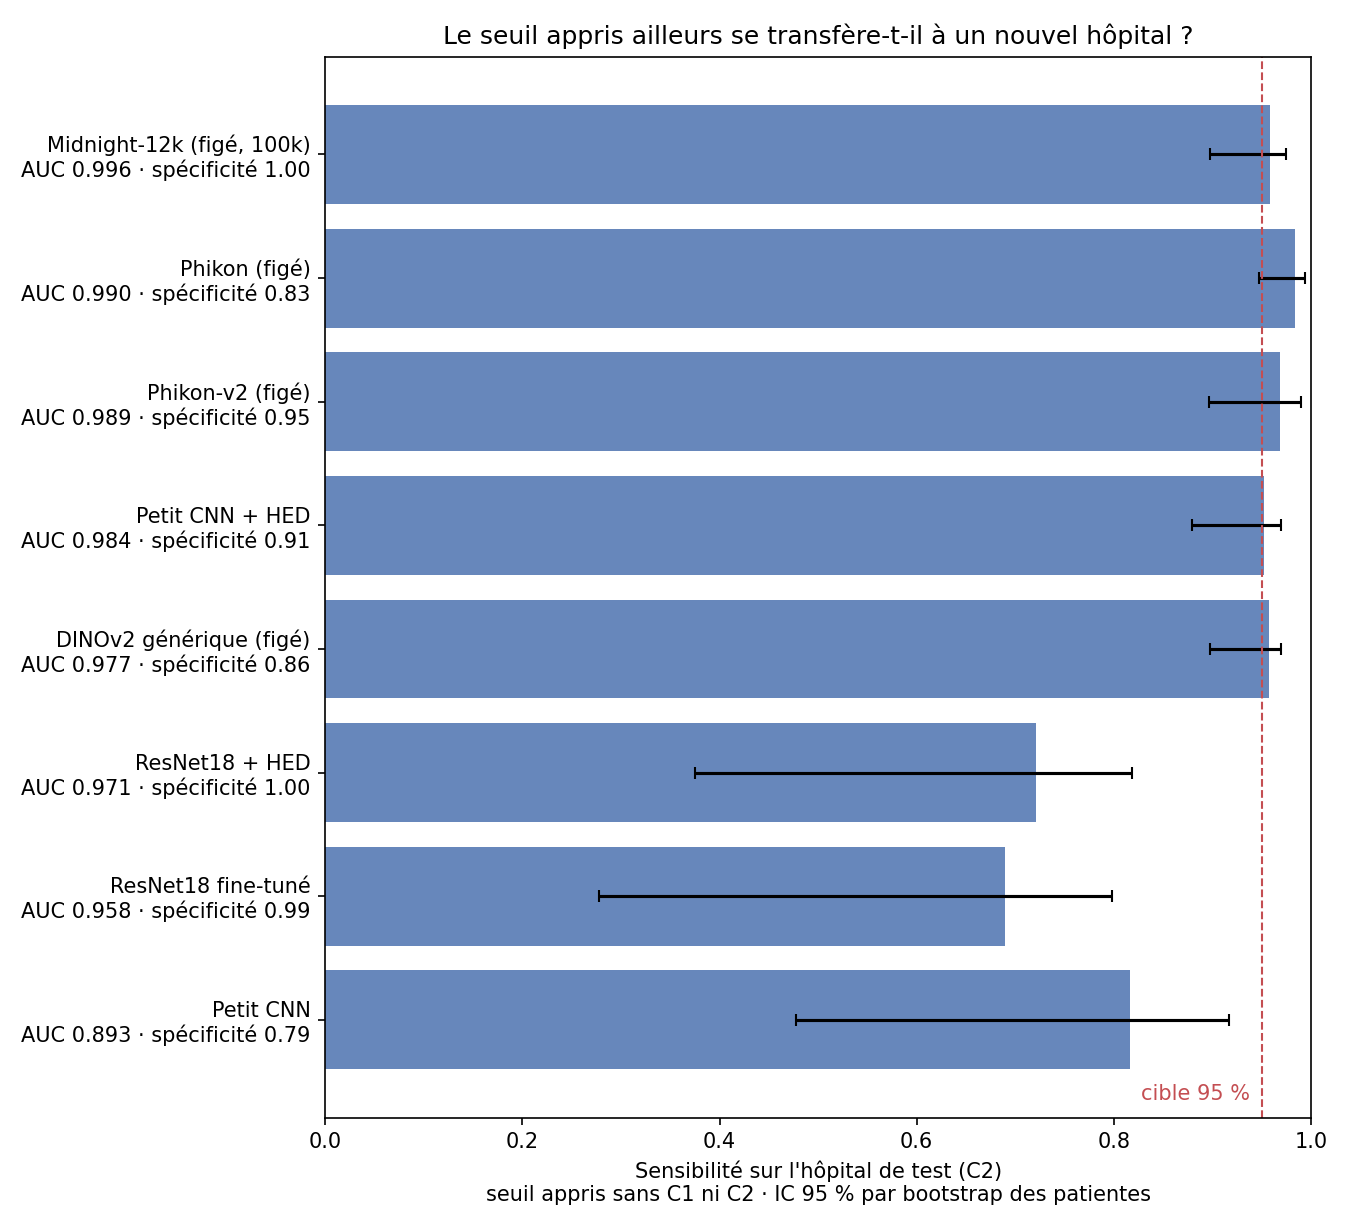
\includegraphics[width=0.74\textwidth]{sensibilite_c2.png}
\caption{Sensibilité sur l'hôpital 2 au seuil appris sans les hôpitaux 1 et 2 (IC 95\,\% par bootstrap des patientes).}
\label{fig:sens}
\end{figure}

\begin{constat}[{Avec un modèle de pathologie, le seuil se transfère}]
\begin{enumerate}
  \item Réglé à 95\,\% sur les hôpitaux d'entraînement, le seuil des sondes donne \textbf{95 à 98\,\%} de sensibilité sur les deux
        hôpitaux inconnus ; le ResNet18 tombe à 69\,\%, avec un IC très large (28–80\,\%) : son comportement dépend des patientes.
  \item Une simple régression logistique sur des caractéristiques \emph{figées} bat un ResNet18 entraîné de bout en bout.
  \item Le pré-entraînement \emph{en pathologie} compte : DINOv2 (photos) transfère aussi son seuil, mais avec plus de fausses alertes.
  \item Phikon, Phikon-v2 et Midnight ont des IC qui se chevauchent : pas de vainqueur net. \textbf{Phikon est retenu} pour l'étape 2,
        car il est le plus rapide (3 millions de tuiles à encoder) ; Midnight offre le meilleur compromis (quasi aucune fausse alerte).
\end{enumerate}
\end{constat}

\subsection{Synthèse de la comparaison des modèles de détection}
\begin{table}[H]
\centering\footnotesize\setlength{\tabcolsep}{3.5pt}
\begin{tabularx}{\textwidth}{lllccX}
\toprule
\textbf{Famille} & \textbf{Modèle} & \textbf{Paramètres appris} & \textbf{AUC C2} & \textbf{Sens. C2} & \textbf{Verdict} \\
\midrule
Classique & Rég. logistique couleur + texture & quelques centaines & 0,660 & 0,63 & s'appuie sur la couleur : ne transfère pas \\
Classique & Forêt aléatoire couleur + texture & 300 arbres & 0,896 & 0,99 & sensible mais 64\,\% de fausses alertes \\
CNN & Petit CNN (de zéro) & 389\,k & 0,893 & 0,82 & simple, mais rangement moyen hors domaine \\
CNN & ResNet18 (ImageNet, fine-tuné) & 11\,M & 0,958 & 0,69 & bon rangement, seuil non transférable \\
CNN & Petit CNN + HED-light & 389\,k & 0,984 & 0,95 & \textbf{gain net} de l'augmentation de couleur \\
CNN & ResNet18 + HED-light & 11\,M & 0,971 & 0,72 & seuil toujours non transférable \\
Fondation & DINOv2-base figé + sonde & 769 (sonde) & 0,977 & 0,96 & transfère, plus de fausses alertes \\
Fondation & \textbf{Phikon figé + sonde} & 769 (sonde) & 0,990 & \best{0,98} & \textbf{retenu} : robuste et rapide \\
Fondation & Phikon-v2 figé + sonde & 1\,025 (sonde) & 0,989 & 0,97 & équivalent, plus lent \\
Fondation & Midnight-12k figé + sonde & $\approx$\,3\,k (sonde) & \best{0,996} & 0,96 & meilleur compromis, très lent \\
\bottomrule
\end{tabularx}
\caption{Les huit classifieurs comparés sur l'hôpital de test, plus deux variantes avec augmentation de couleur (section~\ref{sec:hed}). Les modèles de fondation (86\,M à plus d'un milliard de paramètres)
restent figés : seule la régression logistique est apprise.}
\label{tab:synthese}
\end{table}

%=====================================================================
\section{Résultats — étape 2 : stade pN de 57 patientes}
%=====================================================================

\begin{table}[H]
\centering\footnotesize\setlength{\tabcolsep}{2.5pt}
\begin{tabular}{lccccc}
\toprule
\textbf{Méthode} & \textbf{Kappa (min–max)} & \textbf{pN exact} & \textbf{Métast. ratées} & \textbf{Macro ratées} & \textbf{Sur-stadif.} \\
\midrule
Règle de taille & 0,80 (0,77–0,83) & 69\,\% & 6,4 & 2,1 & 5,4 \\
Forêt aléatoire & 0,80 (0,76–0,87) & 69\,\% & 6,3 & 0,5 & 4,4 \\
ABMIL 3 classes & 0,87 (0,85–0,91) & 78\,\% & 5,1 & 1,3 & \best{1,2} \\
\rowcolor{bleuclair}\textbf{ABMIL hybride (principal)} & \best{0,89} (0,86–0,93) & 79\,\% & \best{4,4} & 2,1 & 1,5 \\
ABMIL hybride, 3 graines & 0,88 (0,86–0,90) & 78\,\% & 4,8 & 2,1 & 1,4 \\
\midrule
\textit{Exploratoire : ABMIL « ET » forêt} & \best{0,89} (0,88–0,91) & \best{81\,\%} & 4,8 & \best{0,3} & 1,4 \\
\bottomrule
\end{tabular}
\caption{3 plis $\times$ 10 répétitions, mêmes plis pour toutes les méthodes ; métriques cliniques en nombre moyen de patientes sur 57.
« ET » : macro si la forêt dit macro \emph{et} l'ABMIL dit « atteint ».}
\label{tab:pn}
\end{table}

\begin{table}[H]
\centering\small
\begin{tabular}{l|ccccc}
\toprule
\textbf{Vérité $\backslash$ prédiction} & pN0 & pN0(i+) & pN1mi & pN1 & pN2 \\
\midrule
pN0 (24) & \textbf{20} & 1 & 3 & 0 & 0 \\
pN0(i+) (3) & 2 & \textbf{0} & 1 & 0 & 0 \\
pN1mi (9) & 6 & 0 & \textbf{2} & 1 & 0 \\
pN1 (14) & 0 & 0 & 0 & \textbf{13} & 1 \\
pN2 (7) & 0 & 0 & 0 & 2 & \textbf{5} \\
\bottomrule
\end{tabular}
\caption{Matrice de confusion du stade pN (forêt aléatoire, une répétition). Les erreurs sont surtout d'un cran ; les pN1mi sont
le plus souvent classées pN0.}
\label{tab:confpn}
\end{table}

\noindent Écarts de kappa appariés [IC 95\,\%] : ABMIL hybride $-$ règle $+0{,}09$ [0,01 ; 0,18] ; ABMIL hybride $-$ forêt
$+0{,}08$ [0,01 ; 0,18] ; ABMIL 3 classes $-$ règle $+0{,}07$ [$-0{,}00$ ; 0,16] ; 3 graines $-$ 1 graine $-0{,}005$ [$-0{,}016$ ; 0,003].

\begin{constat}[Constats de l'étape 2]
\begin{enumerate}
  \item \textbf{L'ABMIL hybride bat la règle et la forêt dans 10 répétitions sur 10}, avec un IC qui exclut 0 (borne basse proche de 0 :
        57 patientes). Le gain vient des petites métastases mieux détectées et de 3 fois moins de fausses alertes.
  \item La forêt rate moins de macro-métastases (0,5 contre 2,1). La combinaison « ET » garde le meilleur des deux (0,3 macro ratée),
        mais elle a été imaginée \emph{après} les résultats : \textbf{exploratoire}, à confirmer sur d'autres patientes.
  \item Moyenner 3 graines n'apporte rien (résultat négatif) ; les cancers avancés sont bien classés (pN1 : 13/14).
  \item \textbf{Point faible : micro-métastases et ITC.} Aucune ITC détectée (plus petite qu'une tuile de 93\,µm) ; 4 à 5 pN1mi
        classées pN0. Repère : les meilleures équipes du challenge atteignaient un kappa d'environ 0,9 sur 500 lames de test, à une
        résolution 4 fois plus fine — non directement comparable.
\end{enumerate}
\end{constat}

%=====================================================================
\section{Changement de domaine}\label{sec:domaine}
%=====================================================================

\subsection{Ce que nous avons mesuré}
\begin{enumerate}
  \item \textbf{La cause} : la couleur seule identifie l'hôpital dans 80\,\% des cas ; l'hôpital 2 est le plus violet.
  \item \textbf{L'effet sur le rangement} : l'AUC des CNN baisse de 0,99 (hôpitaux connus) à 0,91–0,98 (hôpitaux inconnus).
  \item \textbf{L'effet sur la décision}, le plus grave : la sensibilité au seuil transféré tombe à 69\,\% (ResNet18). Le ResNet18
        reste capable de séparer les classes sur l'hôpital 2, mais ses probabilités sont décalées : c'est un problème de
        \emph{calibration} propre à chaque hôpital. Régler le seuil sur l'autre hôpital inconnu (C1) n'aide presque pas (69 $\to$ 74\,\%).
  \item \textbf{Le rôle de la durée d'entraînement} : plus d'époques améliorent \texttt{val\_id} mais dégradent l'hôpital 1. Sur
        l'échantillon du notebook pédagogique (19\,254 patchs), un petit CNN entraîné 300 époques atteint 0,999 d'AUC sur
        \texttt{val\_id} mais ne détecte plus que 35\,\% des tumeurs de l'hôpital 2 : son seuil monte à 0,97 car il est devenu
        très confiant sur ses propres hôpitaux.
\end{enumerate}

\subsection{Le changement de domaine au niveau de la patiente}
Le kappa par hôpital (forêt / règle de taille, 10 à 13 patientes par hôpital) varie de 0,53 à 0,92 : C0 0,82 / 0,80 ; C1 0,78 / 0,57 ;
C2 0,53 / 0,68 ; C3 0,92 / 0,79 ; C4 0,92 / 0,86. L'hôpital 2, le plus violet, reste le plus difficile même avec Phikon, mais ces
chiffres reposent sur une dizaine de patientes et sont très instables : ils indiquent une tendance, pas une conclusion.

\subsection{Deux remèdes testés}\label{sec:hed}
\paragraph{(1) Changer de représentation : modèles de fondation.} C'est le remède le plus efficace (tableau~\ref{tab:fm}) : un
encodeur pré-entraîné sur des millions de patchs de nombreux hôpitaux a déjà vu une grande variété de colorations.

\paragraph{(2) Augmentation de couleur HED-light (exploratoire).}
\emph{Plan fixé et critiqué avant lancement.} Nous ré-entraînons le petit CNN et le ResNet18 sur le jeu complet avec
\textbf{exactement} les mêmes réglages, la même graine et le même découpage que les runs de référence ; seule différence : à chaque lot,
chaque patch est décomposé en ses colorants (déconvolution de Ruifrok : hématoxyline, éosine, résidu), chaque canal est multiplié par
$\alpha\sim\mathcal U[0{,}95 ; 1{,}05]$ et décalé de $\beta\sim\mathcal U[-0{,}05 ; 0{,}05]$, puis l'image est recomposée
(\emph{HED-light}, Tellez et al., 2019). L'intensité n'a pas été réglée au vu des résultats. L'opération est faite par lot sur le GPU
(écart maximal avec scikit-image : $2\cdot10^{-7}$), sans surcoût mesurable ($\approx$\,270\,s par époque).
Critère principal annoncé : l'hôpital 1 ; l'hôpital 2 est regardé une fois. Écarts HED $-$ référence avec IC 95\,\% par
\textbf{bootstrap apparié des patientes} (mêmes tirages pour les deux modèles). Diagnostic supplémentaire : la spécificité au seuil
« oracle » qui donnerait 95\,\% de sensibilité sur l'hôpital lui-même (inutilisable en pratique, mais il isole la séparabilité du
problème de seuil).

\begin{table}[H]
\centering\footnotesize\setlength{\tabcolsep}{3pt}
\begin{tabular}{llcccc}
\toprule
\textbf{Modèle} & \textbf{Hôpital} & \textbf{AUC} & \textbf{Sensibilité} & \textbf{Spécificité} & \textbf{Spéc. au seuil oracle} \\
\midrule
\multirow{2}{*}{Petit CNN} & C1 & 0,912 $\to$ 0,966 & 0,90 $\to$ 0,89 & 0,72 $\to$ \best{0,94} & 0,56 $\to$ 0,82 \\
 & & {\scriptsize +0,05 [$-$0,01 ; 0,22]} & {\scriptsize $-$0,01 [$-$0,12 ; 0,23]} & {\scriptsize \best{+0,23 [0,16 ; 0,33]}} & {\scriptsize +0,26 [$-$0,07 ; 0,45]} \\
 & C2 & 0,893 $\to$ \best{0,984} & 0,82 $\to$ \best{0,95} & 0,79 $\to$ \best{0,92} & 0,59 $\to$ \best{0,92} \\
 & & {\scriptsize \best{+0,09 [0,04 ; 0,23]}} & {\scriptsize \best{+0,14 [0,03 ; 0,45]}} & {\scriptsize \best{+0,12 [0,09 ; 0,15]}} & {\scriptsize \best{+0,33 [0,16 ; 0,48]}} \\
\midrule
\multirow{2}{*}{ResNet18} & C1 & 0,979 $\to$ 0,985 & 0,93 $\to$ 0,88 & 0,91 $\to$ \best{0,99} & 0,88 $\to$ 0,92 \\
 & & {\scriptsize +0,01 [$-$0,00 ; 0,03]} & {\scriptsize $-$0,05 [$-$0,08 ; 0,03]} & {\scriptsize \best{+0,08 [0,05 ; 0,10]}} & {\scriptsize +0,04 [$-$0,02 ; 0,13]} \\
 & C2 & 0,958 $\to$ 0,971 & 0,69 $\to$ 0,72 & 0,99 $\to$ 1,00 & 0,76 $\to$ 0,81 \\
 & & {\scriptsize \best{+0,01 [0,00 ; 0,06]}} & {\scriptsize +0,03 [$-$0,03 ; 0,11]} & {\scriptsize \best{+0,01 [0,00 ; 0,01]}} & {\scriptsize \best{+0,06 [0,01 ; 0,30]}} \\
\bottomrule
\end{tabular}
\caption{Référence $\to$ avec HED-light, puis écart [IC 95\,\% apparié] ; en gras, les écarts dont l'IC exclut 0. Seuils fixés sur
\texttt{val\_id} : petit CNN 0,327 $\to$ 0,305, ResNet18 0,843 $\to$ 0,890.}
\label{tab:hed}
\end{table}

\begin{constat}[{Une augmentation de couleur légère aide nettement le petit CNN, peu le ResNet18}]
\begin{enumerate}
  \item \textbf{Petit CNN} : sur l'hôpital 2, l'AUC passe de 0,893 à \textbf{0,984} et la sensibilité au seuil transféré de 0,82 à
        \textbf{0,95}, avec 2,4 fois moins de fausses alertes : il rejoint le niveau de DINOv2 et s'approche de Phikon
        (figure~\ref{fig:sens}). Sur l'hôpital 1 (critère principal), le gain net porte sur la spécificité (+0,23) ; l'AUC
        progresse sans que l'IC exclue 0.
  \item \textbf{ResNet18} : l'AUC progresse peu (+0,01) et la sensibilité sur l'hôpital 2 reste à 0,72 [0,38–0,82] : son
        \textbf{problème de seuil persiste}. En revanche, l'augmentation supprime la spécialisation au fil des époques : l'AUC sur
        l'hôpital 1 monte de 0,984 à 0,985 au lieu de baisser de 0,983 à 0,958.
  \item Le seuil oracle progresse aussi : la HED améliore la \emph{séparabilité} des classes, pas seulement leur position par rapport au seuil.
  \item Au niveau patiente, le ResNet18 + HED ne détecte aucun patch tumoral chez 1 des 9 patientes de l'hôpital 2 (0 sans HED) ;
        le petit CNN passe de 1 à 0 patiente entièrement ratée.
\end{enumerate}
\textbf{Statut : exploratoire} (une graine, \texttt{val\_id} de 5 patientes, 8–9 patientes par hôpital externe). La HED réduit
le problème de couleur à moindre coût, mais seuls les modèles de fondation atteignent environ 95\,\% de sensibilité sur les
\emph{deux} hôpitaux inconnus (le petit CNN + HED reste à 0,89 sur l'hôpital 1).
\end{constat}


%=====================================================================
\section{Interprétabilité}
%=====================================================================

\paragraph{Grad-CAM sur le ResNet18.} Pour comprendre les 31\,\% de tumeurs ratées sur l'hôpital 2, nous calculons des cartes
Grad-CAM (Selvaraju et al., 2017) sur la couche \texttt{layer3} (figure~\ref{fig:gradcam}).

\begin{figure}[H]
\centering
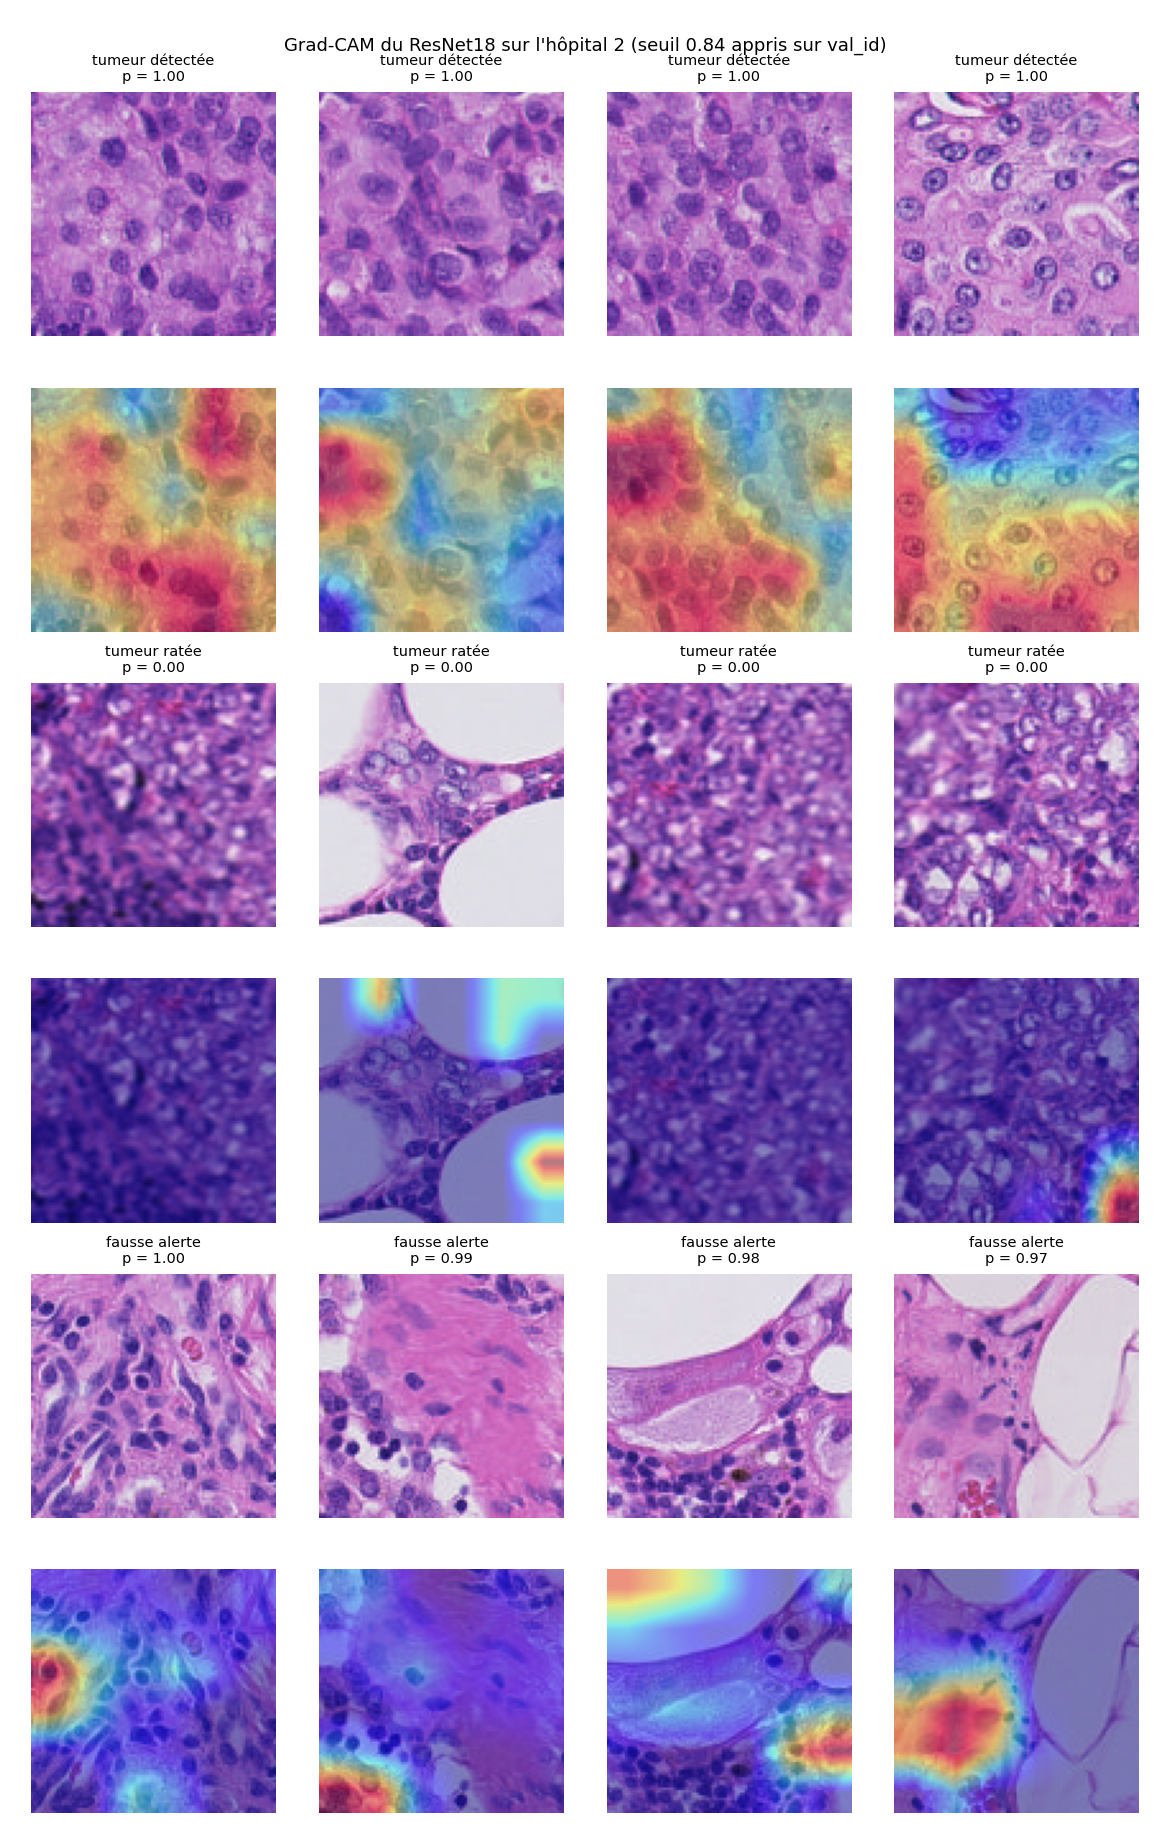
\includegraphics[width=0.49\textwidth]{gradcam_c2_ref.png}\hfill
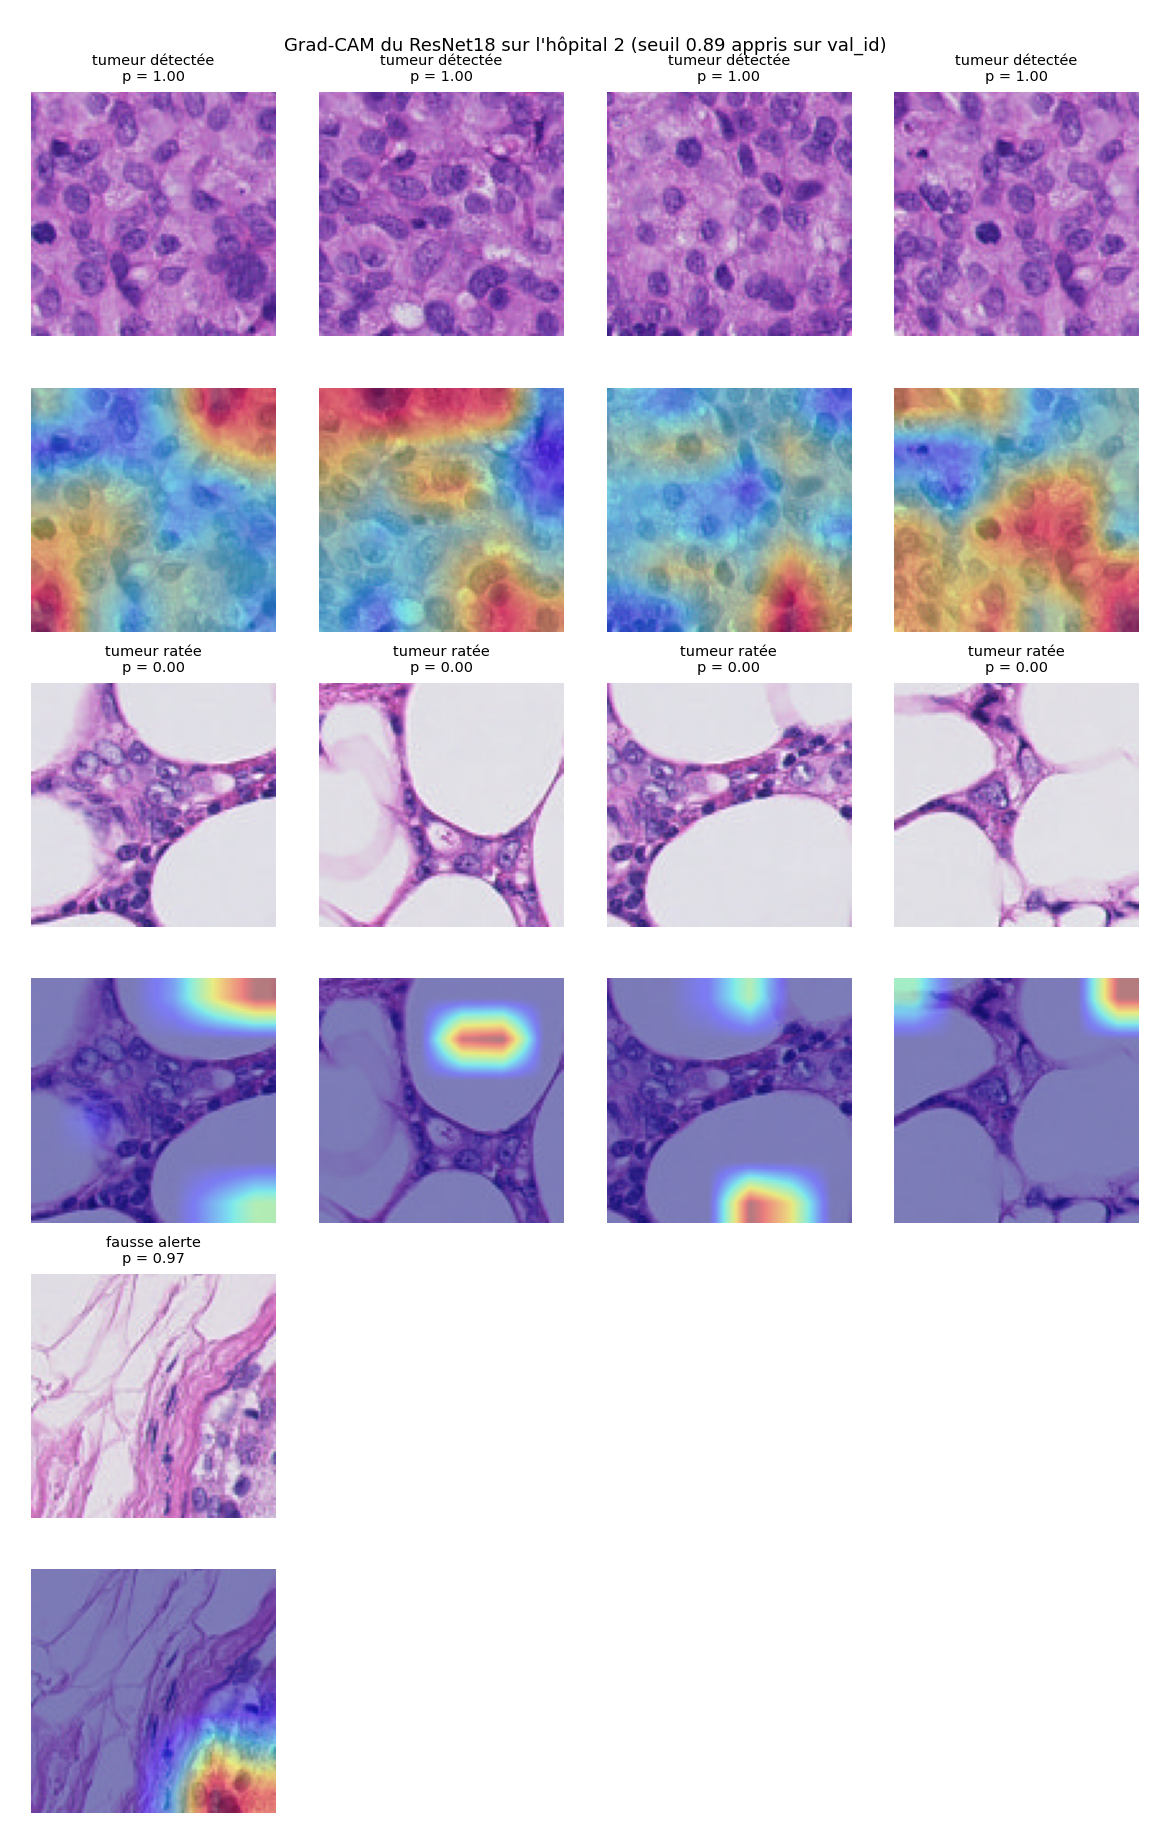
\includegraphics[width=0.49\textwidth]{gradcam_c2_hed.png}
\caption{Grad-CAM du ResNet18 sur 3\,000 patchs de l'hôpital 2, sans (à gauche) et avec augmentation HED (à droite) ; rouge : zones
qui poussent vers « tumeur ». Par groupe : tumeurs détectées, tumeurs ratées, fausses alertes (le modèle HED n'en fait qu'une sur
cet échantillon).}
\label{fig:gradcam}
\end{figure}

\noindent \textbf{Lecture.} Sur les tumeurs détectées, l'activation couvre les amas de grands noyaux irréguliers : le modèle regarde la
bonne morphologie. Les tumeurs ratées les plus franches ($p\approx0$) sont des patchs \textbf{très sombres, saturés et flous} : la
carte est presque vide, le modèle n'y trouve aucun indice de tumeur. C'est cohérent avec le décalage de couleur de l'hôpital 2 :
hors de la plage de couleurs vue à l'entraînement, les motifs appris ne s'activent plus. Les fausses alertes s'allument sur des
amas de noyaux denses ou des cellules endothéliales en bord de graisse, confusions plausibles même pour un œil humain.
\textbf{Avec l'augmentation HED}, les tumeurs ratées les plus franches ne sont plus des patchs sombres et saturés, mais quelques cellules
tumorales isolées entre de grandes vacuoles de graisse : l'erreur devient \emph{morphologique} (peu de cellules), et non plus liée à
la couleur. C'est un argument qualitatif en faveur de l'effet attendu de l'augmentation.

\paragraph{Cartes de chaleur et attention (étape 2).} La carte de chaleur d'une lame entière permet au pathologiste de vérifier
\emph{où} le modèle voit une métastase et de mesurer la taille de la lésion, comme la règle de taille. Les erreurs typiques
(figure~\ref{fig:cartes}) sont des micro-métastases trop petites pour colorer plus de quelques tuiles, et des fausses alertes isolées.
L'ABMIL fournit en plus des poids d'attention par tuile.

\begin{figure}[H]
\centering
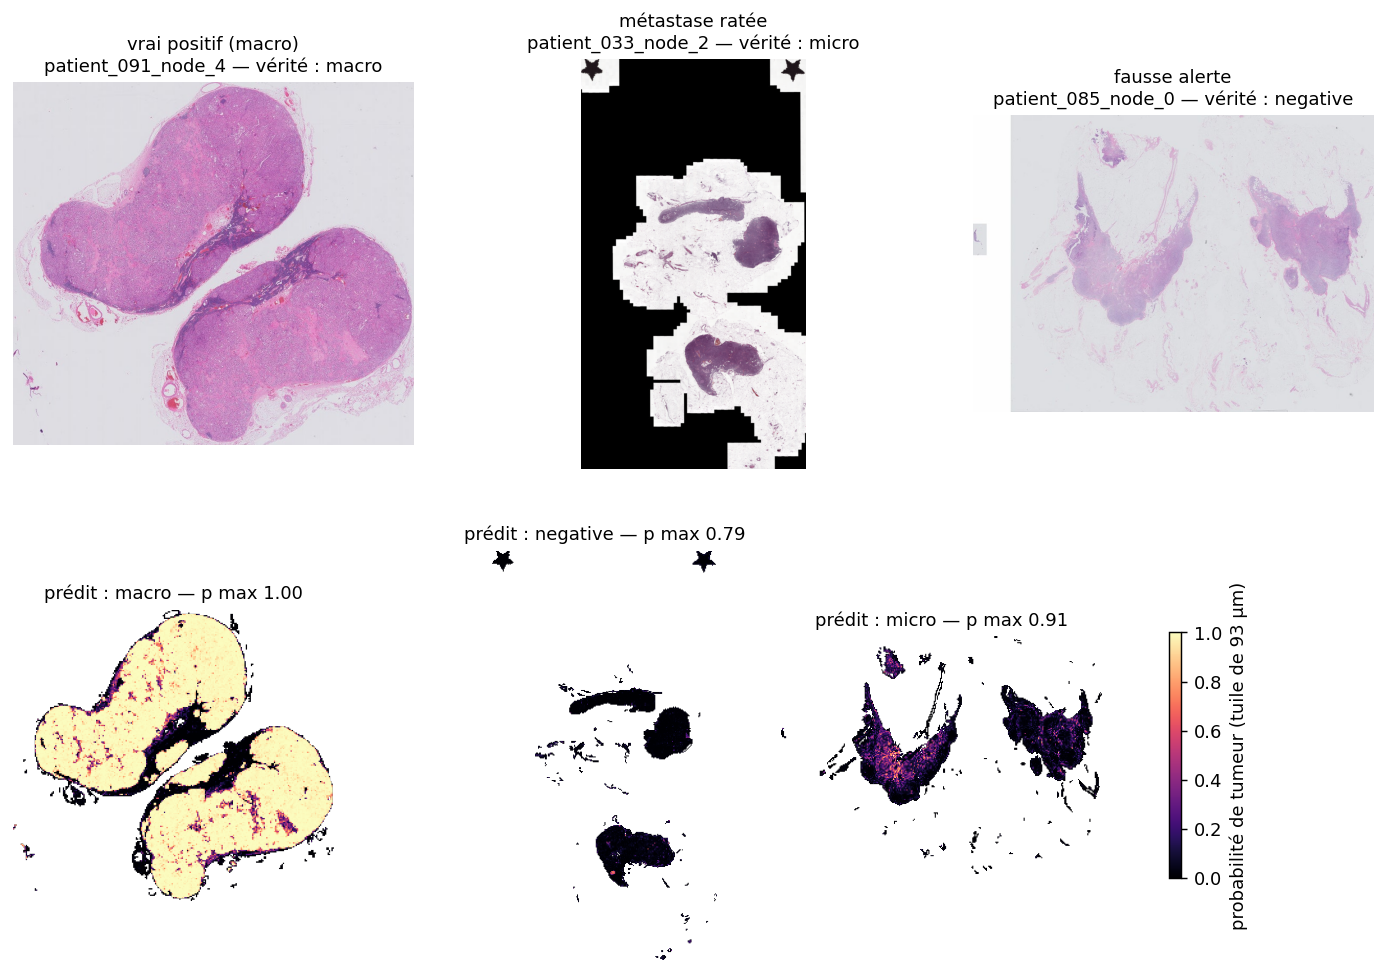
\includegraphics[width=0.92\textwidth]{pn_cartes_exemples.png}
\caption{Cartes de chaleur Phikon + sonde sur des lames de la cohorte pN : vrai positif, métastase ratée, fausse alerte.}
\label{fig:cartes}
\end{figure}

\begin{limite}[Limites de ces explications]
Grad-CAM et l'attention montrent \emph{où} se porte la décision, pas \emph{pourquoi} : ce sont des corrélations, pas des explications
causales. Les exemples présentés sont choisis parmi les cas extrêmes et ne représentent pas toute la distribution. En revanche, la
règle de taille et la chaîne « carte $\to$ diamètre $\to$ règles TNM » sont explicables par construction.
\end{limite}

%=====================================================================
\section{Éthique et usage responsable}
%=====================================================================
\begin{itemize}
  \item \textbf{Un outil d'aide, pas de remplacement.} Le système doit trier et signaler, la décision restant au pathologiste. Notre
        protocole de relecture le montre : relire les 22\,\% de patientes où ABMIL et forêt ne sont pas d'accord rattrape presque toutes
        les macro-métastases restantes, mais \textbf{pas les micro-métastases} : les lames jugées négatives doivent rester relues.
  \item \textbf{Coût asymétrique.} Nous privilégions la sensibilité, au prix de fausses alertes : c'est un choix de valeurs qui doit être
        explicite, discuté avec les cliniciens, et non caché dans un seuil à 0,5.
  \item \textbf{Biais et généralisation.} Les données viennent de 5 hôpitaux néerlandais, d'une population et de protocoles de coloration
        limités. Nos résultats montrent qu'un modèle excellent chez lui peut rater un tiers des tumeurs ailleurs : \textbf{toute mise
        en service exige une validation locale}, hôpital par hôpital, et une surveillance continue (dérive de scanner ou de coloration).
  \item \textbf{Transparence des performances.} Rapporter l'AUC seule serait trompeur ; nous rapportons la sensibilité au seuil
        transféré, les intervalles de confiance et les résultats négatifs.
  \item \textbf{Données de santé.} Les données sont publiques et anonymisées ; un déploiement réel relèverait du RGPD (données de santé),
        de l'hébergement certifié et, pour un logiciel d'aide au diagnostic, du règlement européen sur les dispositifs médicaux et de
        l'AI Act (système à haut risque).
  \item \textbf{Responsabilité et confiance.} En cas d'erreur, la responsabilité doit rester identifiable ; les cartes de chaleur aident le
        médecin à garder un regard critique et évitent la confiance aveugle (biais d'automatisation).
  \item \textbf{Licences et outils.} Les modèles de fondation utilisés ont des licences de recherche ; une partie du code a été écrite avec
        l'aide d'un assistant d'IA (Claude), relue et comprise par l'équipe.
\end{itemize}

%=====================================================================
\section{Conclusion, limites et perspectives}
%=====================================================================

\paragraph{Ce que nous retenons.}
\begin{enumerate}
  \item \textbf{Comparer les modèles sur un hôpital jamais vu change le classement.} Sur les hôpitaux d'entraînement, tous les CNN
        semblent excellents ; sur un hôpital inconnu, seul un encodeur pré-entraîné en pathologie garde une sensibilité proche de 95\,\%.
  \item \textbf{L'AUC ne suffit pas} : il faut évaluer la décision, au seuil réellement utilisable.
  \item \textbf{Deux remèdes au changement de domaine} : changer de représentation (modèles de fondation, le plus efficace) ou
        augmenter la couleur à l'entraînement (efficace pour le petit CNN, insuffisant pour le ResNet18, résultat exploratoire).
  \item \textbf{Modèles retenus} : Phikon figé + régression logistique pour la détection ; ABMIL hybride pour le stade pN (kappa 0,89).
\end{enumerate}

\begin{limite}[Limites]
\begin{itemize}
  \item Peu de patientes : 8–9 par hôpital externe à l'étape 1, 57 à l'étape 2 ; les IC sont larges.
  \item L'hôpital 2 a été regardé pour plusieurs modèles : ces comparaisons sont descriptives ; le choix du modèle repose sur la
        validation croisée et l'hôpital 1.
  \item Les CNN, avec ou sans HED, n'ont été entraînés qu'avec une graine ; les réglages de l'étape 2 sont choisis dans la validation croisée.
  \item La vérité « taille » des pathologistes vient de l'immunohistochimie, que le modèle ne voit pas ; notre résolution (1\,µm/pixel)
        est 4 fois plus grossière que celle des gagnants du challenge.
\end{itemize}
\end{limite}

\paragraph{Perspectives.} (1) Relire à plus haute résolution les seules zones suspectes, pour les micro-métastases ;
(2) encodeurs plus récents (UNI, CONCH, Virchow) ; (3) confirmer l'effet de la HED avec plusieurs graines, tester une intensité plus forte et la normalisation de
coloration (Macenko), choisies sur l'hôpital 1 ; (4) validation sur de nouvelles patientes avant de confirmer la combinaison « ET ».

\section*{Références}
\small
\noindent Bándi P. et al. (2019). From detection of individual metastases to classification of lymph node status at the patient level:
the CAMELYON17 challenge. \emph{IEEE TMI}.\\
Koh P.W. et al. (2021). WILDS: a benchmark of in-the-wild distribution shifts. \emph{ICML}.\\
He K. et al. (2016). Deep residual learning for image recognition. \emph{CVPR}.\\
Filiot A. et al. (2023). Scaling self-supervised learning for histopathology with masked image modeling (Phikon). \emph{medRxiv}.\\
Oquab M. et al. (2023). DINOv2: learning robust visual features without supervision. \emph{arXiv}.\\
Ilse M., Tomczak J., Welling M. (2018). Attention-based deep multiple instance learning. \emph{ICML}.\\
Tellez D. et al. (2019). Quantifying the effects of data augmentation and stain color normalization in convolutional neural networks
for computational pathology. \emph{Medical Image Analysis}.\\
Selvaraju R.R. et al. (2017). Grad-CAM: visual explanations from deep networks via gradient-based localization. \emph{ICCV}.\\
Macenko M. et al. (2009). A method for normalizing histology slides for quantitative analysis. \emph{ISBI}.

\end{document}
